\documentclass{article}

\usepackage{siunitx} % Provides the \SI{}{} and \si{} command for typesetting SI units

\usepackage{graphicx} % Required for the inclusion of images

\usepackage{tabularx} % Tables

\usepackage{natbib} % Required to change bibliography style to APA
\usepackage{float}
\usepackage{hyperref}
\usepackage[normalem]{ulem}
\useunder{\uline}{\ul}{}

\usepackage{amsmath} % Required for some math elements

% Many options for pseudocode
\usepackage{algorithm2e}
\usepackage{algorithmic}

\usepackage{listings} % Python code blocks
\usepackage[margin=1in]{geometry} % CUSTOM

\setlength\parindent{0pt} % Removes all indentation from paragraphs

\title{Lab 5 Report: Localization on the Racecar} % Title

\author{Team 22 \\\\ Benjamin Rich \\ Dinuri Rupasinghe \\ Sophia Wang \\ Steven Liu \\ Jose Soto  \\ Editor for Lab 5: Benjamin Rich\\\\ 16.405/6.4200} % Team # + Names, Class (RSS)

\date{\today} % Date for the report
\begin{document}

\maketitle


\tableofcontents
\newpage


\section{Introduction (Author: Sophia Wang)}
% include a description of purpose and lab, define lab goals
% limit 6500 words. Short informal description of technical problem
The purpose of Lab 5: Monte Carlo Localization (MCL) is to determine the robot's orientation and position in a known environment, a critical problem in the field of robotics. Localization is a fundamental functionality required by an autonomous robot since the knowledge of its own location in time is an essential prerequisite to making decisions about future actions, such as path planning. Additionally, the ability to avoid dangerous situations such as collisions and unsafe conditions can be related to specific places in the robot environment. Localization is important both for path planning and obstacle avoidance. \\

We are specified to utilize ROS software given by the course staff of Robotics, Science, and Systems. We will be utilizing the LiDAR sensor data we receive from the racecar, odometry data from the wheels and steering, the racecar router for transferring this data, and built-in ROS packages to implement the Python scripts we will be creating. \\

The goal of this lab is to successfully implement MCL on the racecar to obtain odometry estimates and potential particle locations. MCL is an algorithm for robots to establish position and orientation in a known environment using a particle filter. The algorithm uses a particle filter to represent the distribution of likely states, with each particle representing a possible state. Over time, the estimates of particles' positions converge to the robots true location. \\

We tackle the technical problem by utilizing these main steps: implementing a motion model, implementing a sensor model, and implementing a particle filter. The particle filter uses both the motion model and sensor model to listen to laser and odometry data and publish new odometry data based on adapted particle probabilities and resampling. Throughout each step, we use unit tests where a racecar-simulator with a small testing map is generated, and the robot is placed in a predetermined location. Additionally, when integrating and adjusting the algorithm to hardware, we publish our estimated pose to the simulator for easy comparison with a ground truth map. \\

A challenge in the implementation of MCL is that ROS callbacks are not necessarily threadproof. Additionally, for real-time performance in the racecar, we must publish transformations from the map to the car's position at a rate greater than 20 Hz since at race speeds (~10 meters per second), the poses we publish could be as much as half a meter apart, which could interfere with controller performance. \\

\section{Technical Approach (Author: Dinuri Rupasinghe)}

\subsection{Overview}
The process of implementing Monte Carlo Localization on our racecar includes three main parts: the motion model, the sensor model, and the particle filter. The particle filter will  use the motion model and sensor model to manipulate data from the racecar. Specifically, we will be subscribing to lidar data, odometry data, and inital pose data from the racecar and passing it into the motion model and sensor model. The particle filter will resample probabilities of the car's position and publish a new odometry message estimate and a new transform message.

\subsection{Motion Model (Author: Steven Liu)}

The motion model calculates how pose estimates change based on odometry data measured from the car. In particular, for a given pose (or for each pose in an array of poses), we compose with it a transformation derived from the odometry $\Delta x,\Delta y,\Delta \theta$ in the car frame.

Because we are working in two dimensions, poses consist of three components $x,y,\theta$, representing two Cartesian coordinates and a rotation relative to a fixed world frame. To compute a new pose, we only need to convert the odometry, which is represented relative to the car, to the same frame as the poses. This requires us to rotate the transformation using the rotation matrix \[R_\theta = \left[\begin{matrix}\cos\theta & -\sin\theta \\ \sin\theta & \cos\theta \end{matrix}\right]\] which can be used to rotate the odometry $\Delta x,\Delta y$ into the world frame. $\Delta\theta$ is simpler to handle: we only need to add it to $\theta$ directly. Thus, we get a new pose

\begin{align}
    x' & = x+\Delta x\cos\theta-\Delta y\sin\theta \nonumber \\
    y' & = y+\Delta x\sin\theta+\Delta y\cos\theta \nonumber \\
    \theta' & = \theta+\Delta\theta \nonumber
\end{align}

The computation thus far has been fully deterministic. However, while the odometry is quite good, it is not infinitely accurate. Thus, adding noise to the final pose is desirable. This is accomplished by adding three uncorrelated normally distributed random values to the components $x,y,\theta$ of the final pose.

\subsection{Sensor Model (Author: Benjamin Rich)}
A crucial aspect of Monte Carlo Localization is the ability to approximate the probability of various poses being the actual robot location, given some sort of observation. In the case of our car, a pose is defined by $(x,y,\theta)$ relative to the map frame, and our observation is an array of distances from a scan of our Hokuyo LIDAR. In order to establish the probablity of a pose, we first need to establish the probability of a certain distance being recieved as part of a LIDAR scan. \\

\textbf{LIDAR Distance Probability Distribution}: Multiple distributions are combined into one to create a continuous probability disribution that approximaes the probability of a given LIDAR scan outputting a distance $z_k$ given a hypothesis distance $x_k$. In short, four possible 'events' that could affect the reading are accounted for: 
\begin{enumerate}
    \item The probability of detecting a known obstacle as expected in the map is modeled using a Gaussian distribution ($p_{hit}$) centered a the hypothesis distance (i.e. the Gaussian distribution is maximum at the actual distance). $$p_{hit}(z_{k}^{(i)}| x_{k}, m)  = \begin{cases}
    \eta \frac{1}{\sqrt{2\pi\sigma^2}} \exp\left(-\frac{(z_k^{(i)} - d)^2}{2\sigma^2}\right)  &   \text{if} \quad 0 \leq z_{k} \leq z_{max}\\
    0   &   \text{otherwise}
    \end{cases}$$
    \item The probability of a short measurement caused by LIDAR reflections or other errors is modeled as a downward-sloping distribution ($p_{short}$). $$p_{short}\left(z_{k}^{(i)}| x_{k}, m\right) =  \frac{2}{d} \begin{cases}
         1 - \frac{z_{k}^{(i)}}{d}   &   \text{if} \quad 0 \leq z_{k}^{(i)} \leq d \text{ and } d \neq 0\\
         0   &   \text{otherwise}
\end{cases}$$
    \item The probability of a missed measurement due to a transparent surface or other errors is modeled as a spike in probability at the maximum range $(p_{max})$. $$p_{max}(z_{k}^{(i)} | x_{k}, m) =\begin{cases}
    \frac{1}{\epsilon}  &  \text{if} \quad z_{max} - \epsilon \leq z_k^{(i)} \leq z_{max}\\
    0  &  \text{otherwise} 
    \end{cases}$$ 
    \item The probability of a random measurement is modeled as a small uniform distribution $(p_{rand})$. $$p_{rand}(z_{k}^{(i)} | x_{k}, m)  = \begin{cases}
    \frac{1}{z_{max}}  &  \text{if} \quad 0\leq z_{k}^{(i)} \leq z_{max}\\
    0                            & \text{otherwise} 
    \end{cases}$$
\end{enumerate}
These four distributions are weighted by parameters that sum to one, as in the below equations: 
$$p(z_{k}^{(i)}| x_{k}, m)  = \alpha_{hit} \cdot p_{hit}(z_{k}^{(i)}| x_{k}, m)  + \alpha_{short} \cdot p_{short}(z_{k}^{(i)}| x_{k}, m)  + \alpha_{max} \cdot p_{max}(z_{k}^{(i)}| x_{k}, m)  + \alpha_{rand} \cdot p_{rand}(z_{k}^{(i)}| x_{k}, m)$$
$$\alpha_{hit}+\alpha_{short}+\alpha_{max}+\alpha_{rand}=1$$
In our case, we used the default $\alpha_{hit}=0.74,\alpha_{short}=0.07,\alpha_{max}=0.07,\alpha_{rand}=0.12,\sigma_{hit}=8.0$ as suggested for this lab. \\

A visual of the resulting distribution is shown below in Figure 1:

\textbf{\begin{figure}[H]
\begin{center}
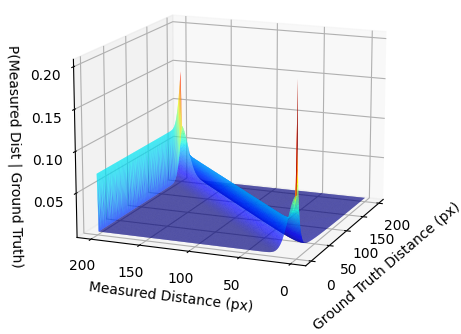
\includegraphics[width=0.5\textwidth]{Sensor_Model_Plotted.png} % Include the image 
\caption{Plot of $p(z_{k}^{(i)}| x_{k}, m)$; the Probability of Receiving a Distance $z_k$ Given a Hypothesis Distance $x_k$. }
\end{center}
\label{workflow}
\end{figure}}

Having the ability to compute this distribution is useful, but the computation time can be high. Instead, we seek to improve computation time via creating a 'look-up' table. \\

\textbf{Discretization and Look-Up Table Creation}: We precompute a table of probabilities, where columns are the actual distance $d$, rows are the measured distance $z_k$, and the value at a given row and column is $p(z_k|d)$. The probabilities are properly normalized across columns such that the probability of all locations given $d$ sum to 1.0. This table allows us to quickly look up the probability of a distance scan given our actual distance. Figure 2 shows a visual image of an example look-up table as described. 

\textbf{\begin{figure}[H]
\begin{center}
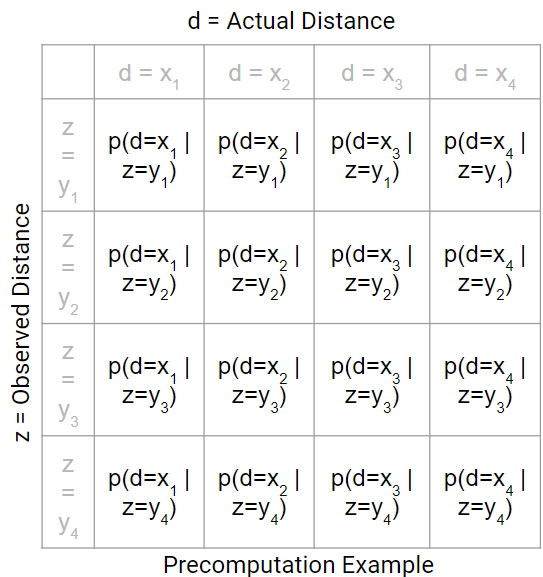
\includegraphics[width=0.3\textwidth]{table.png} % Include the image 
\caption{Example Image Showing a Discretized Probability Look-Up Table. }
\end{center}
\label{workflow}
\end{figure}}
Having created a look-up table, we can finally use it to evaluate the probability of a pose. \\

\textbf{Evaluating the Probability of a Pose}: Given a LIDAR scan (an observation) and several hypothesis poses, we can estimate the probability of each pose. We first generate a simulated LIDAR scan for each pose using ray tracing (i.e. given a position and orientation on the map, and given knowledge of how the LIDAR scan performs a scan, trace points from the LIDAR out to the map to get estimated LIDAR scan distances). Then, we compute the product probability of each distance in a single scan given the actual distance observed, and thus are able to output the probability of each particle being at the robots actual position in the map! A flowchart for this process is shown in Figure 3. 
\textbf{\begin{figure}[H]
\begin{center}
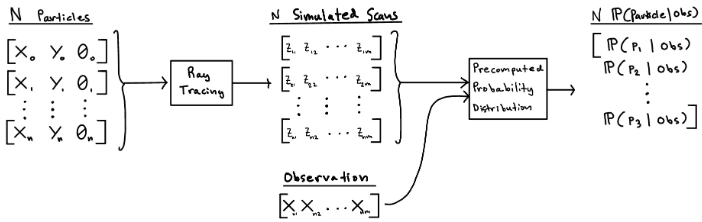
\includegraphics[width=0.8\textwidth]{flowchart.png} % Include the image 
\caption{Flowchart Showing the Process of Computing the Probability of Estimated Poses (Particles) Given observed LIDAR Data. }
\end{center}
\label{workflow}
\end{figure}}

We then implement the above methods in code. \\

\textbf{Details on Code Implementation:} Our sensor model is implemented using a class structure. Upon initialization, the class creates and stores the discretized table. Then, upon receiving a LIDAR scan and poses through a function call, the probability of each pose is computed and returned for use in the particle filter! All processes in the evaluation of probabilities are implemented with numpy matrix operations to avoid significant computation time. 


\subsection{Particle Filter (Author: Dinuri Rupasinghe}
We have implemented a motion model and sensor model. Now, we can implement Monte Carlo Localization by incorporating both of these models into one formal script - this is the particle filter. The particle filter is composed of three main steps. First, we must obtain the initial pose and create a set of initial particles based on this initial pose. Then, we must publish an odometry message when we obtain odometry data and publish an odometry message when we obtain lidar scan data. Below is a diagram of this workflow.
\textbf{\begin{figure}[H]
\begin{center}
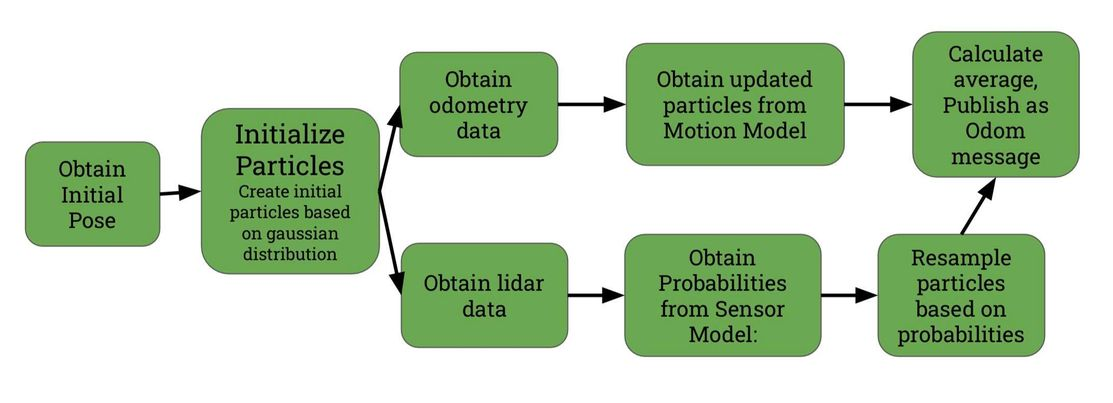
\includegraphics[width=0.8\textwidth]{pf.jpg}
\caption{Diagram of Particle Filter Implementation}
\end{center}
\end{figure}}

\textbf{Initial Pose and Particles}: we are able to access an initial pose of our racecar by accessing the initial pose, of type \emph{PoseWithCovarianceStamped}. In order to access this attribute by placing the car in different positions on our map using a 2D pose estimate, we must add the Pose with Covariance topic in RViz. Thus, we have the ability to access the position and covariance of the initial position. It is important to access this data because it enables us to obtain an inference on an appropriate initial set of particles. \\
\\
In order to generate a random set of initial particles, we used a python numpy function to obtain a random sample of a multivariate normal distribution. Our group chose this specifically because we wanted to create a set of particles based on as much data as possible, and this particular function, \emph{random.multivariatenormal} creates a distribution based on both the initial pose and the covariance of the initial pose.\\

\textbf{Obtain Pose from Motion Model}: One of our goals is to publish new odometry data when the robot obtains odometry data. In order to do this, we utilize our motion model, since we can obtain a new set of particles based on our current set of particles and current odometry data. By recording time between the aggregation of current odometry data and the moment we attempt to calculate new odometry data, we can obtain current odometry data. \\
Once we obtain the most up to date odometry data, we are able to generate a set of updated particles by passing our current particles and current odometry into an evaluate function of our motion model. We then calculate the average of these particles and publish this average as an odometry message and as a pose transform message.\\

\textbf{Obtain Pose from Sensor Model}: Another goal of the particle filter is to generate new odometry data while factoring in the probabilities calculated by the sensor model. We calculate probabilities of each particle's position by using the sensor model's evaluate function and passing in a set of particles and lidar scan data. Then we conduct a resample of the particles. The purpose of resampling is to generate a new set of particles based on particles that are likely to be present. We performed this resample by using the numpy function \emph{random.choice}, and generated particles given the current particles, the amount of particles we desire, and the probabilities calculated by the sensor model. We also inserted a clause stating that there is a thirty percent chance that we return the current version of particles rather than resample based on their probabilities. We implemented this because there is a chance that our racecar does randomly choose the same set of particles again. After resampling, once again, we calculate the average of these updated particles from the resample and publish this average as an odometry message and as a pose transform message.\\

\textbf{Calculating Average of Particles}: As a note, we calculate the x and y averages of our particles as one would calculate them classically. However, we accounted differently for the average of circular coordinates because simply taking the average of the angles will lead to an inaccurate calculation. Instead, we first take the average of the sine and cosine components and then obtain an average angle based on the average sine and cosine, utilizing arctangent. \\

\textbf{Quaternions}: It is important to note that some of the attributes of the data that we subscribe to from the racecar is in the form of quaternions rather than angles in units of degrees. We therefore applied a transformation using an import of \emph{tf.transformations as trans}, which one can see is applied in our code.
%%%% check particle_lock with steven
\\
\\
\textbf{Locking and Threading}: Lastly, a large reason why our simulation ran into errors was because multiple processes were running at once. Since our racecar was retrieving both odometry data and laser scan data at the same time, our particle filter attempted to subscribe to an odometry and lidar callback at the same time. We fixed this by applying a series of "locks". Thus, the both the motion model and the sensor model portions of our particle filter can run sequentially rather than at the same time.

\section{Experimental Evaluation (Author: Benjamin Rich)}
\subsection{Overview}
 Having implemented our motion model, sensor model, and particle filter, we sought to qualify the performance of our MCL implementation in simulation and in real life. To do so we use a three-pronged approach. We qualified our system in simulation using the gradescope autograder provided and we qualitatively tested our system in the Stata basement by making a comprehensible video comparing the performance of our tracking to the actual position. We measured the convergence rate of our particles both on the car and in simulation and measured cross-tracking error in simulation. 

\subsection{Gradescope Autograder}
The Gradescope Autograder provided by staff provides a useful performance metric. In these simulations, our particle filter receives simulated odometry data and laser scans and estimates the position of the car with respect to ground truth. This is done in the presence of no odometry noise, some odometry noise, and more odometry noise. The resultant plots are shown in Figure 4. 

\textbf{\begin{figure}[H]
\begin{center}
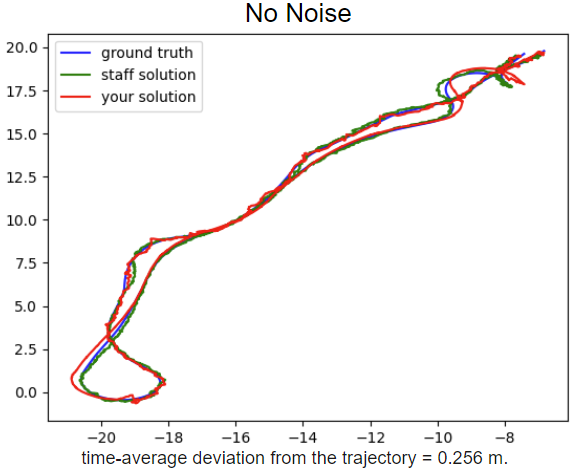
\includegraphics[width=0.45\textwidth]{No_Noise_2.png} % 
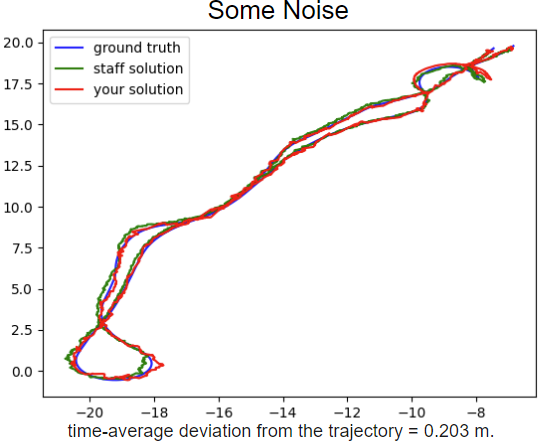
\includegraphics[width=0.45 \textwidth]{Some_Noise_2.png} % 
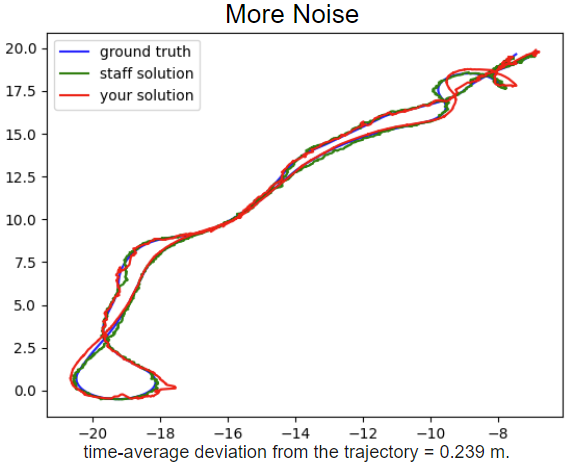
\includegraphics[width=0.45\textwidth]{More_Noise_2.png} % 
\caption{Gradescope Simulation Plots. From left to right, top down: No Odometry Noise, Some Odometry Noise, More Odometry Noise.}
\end{center}
\label{workflow}
\end{figure}}
Visually, our solution performs well. However, we can notice that especially with no or more noise, our solution struggles to track tight turns as well as perhaps it should. This suggests there is room for improvement in our motion model for how it handles tight turns. For each simulation as shown in Figure 4, Gradescope provides a time-averaged deviation from the trajectory. These results are summarized in Table 1. \\
\begin{center}
\begin{tabular}{|l|c|c|c|}
\hline
\textbf{Experiment}                                                    & No Noise & Some Noise & More Noise \\ \hline
\multicolumn{1}{|c|}{\textbf{Time-Averaged Deviation from Trajectory}} & 0.256m   & 0.203m     & 0.239m     \\ \hline
\end{tabular}
\end{center}
These values are good, but not great. A deviation of $0.2-0.26$m or of $0.66-0.84$ feet may be acceptable for some applications but certainly could be too high in situations that require higher precision (such as navigating a complex area). However, in practice, we found this deviation to be not very noticeable. 


\subsection{Video Demonstration}
A video demonstration of MCL in the Stata Basement was creative for the purposes of qualitative observation-based evaluation of our performance. The video can be accessed at: \\

\begin{center}
    \href{https://drive.google.com/file/d/1GLzSGjiPZLCoxgMg-a0pmlcAc0vJkYSs/view?usp=sharing}{https://drive.google.com/file/d/1GLzSGjiPZLCoxgMg-a0pmlcAc0vJkYSs/view?usp=sharing}
\end{center}

An example frame from our video is shown in Figure 5. 

\textbf{\begin{figure}[H]
\begin{center}
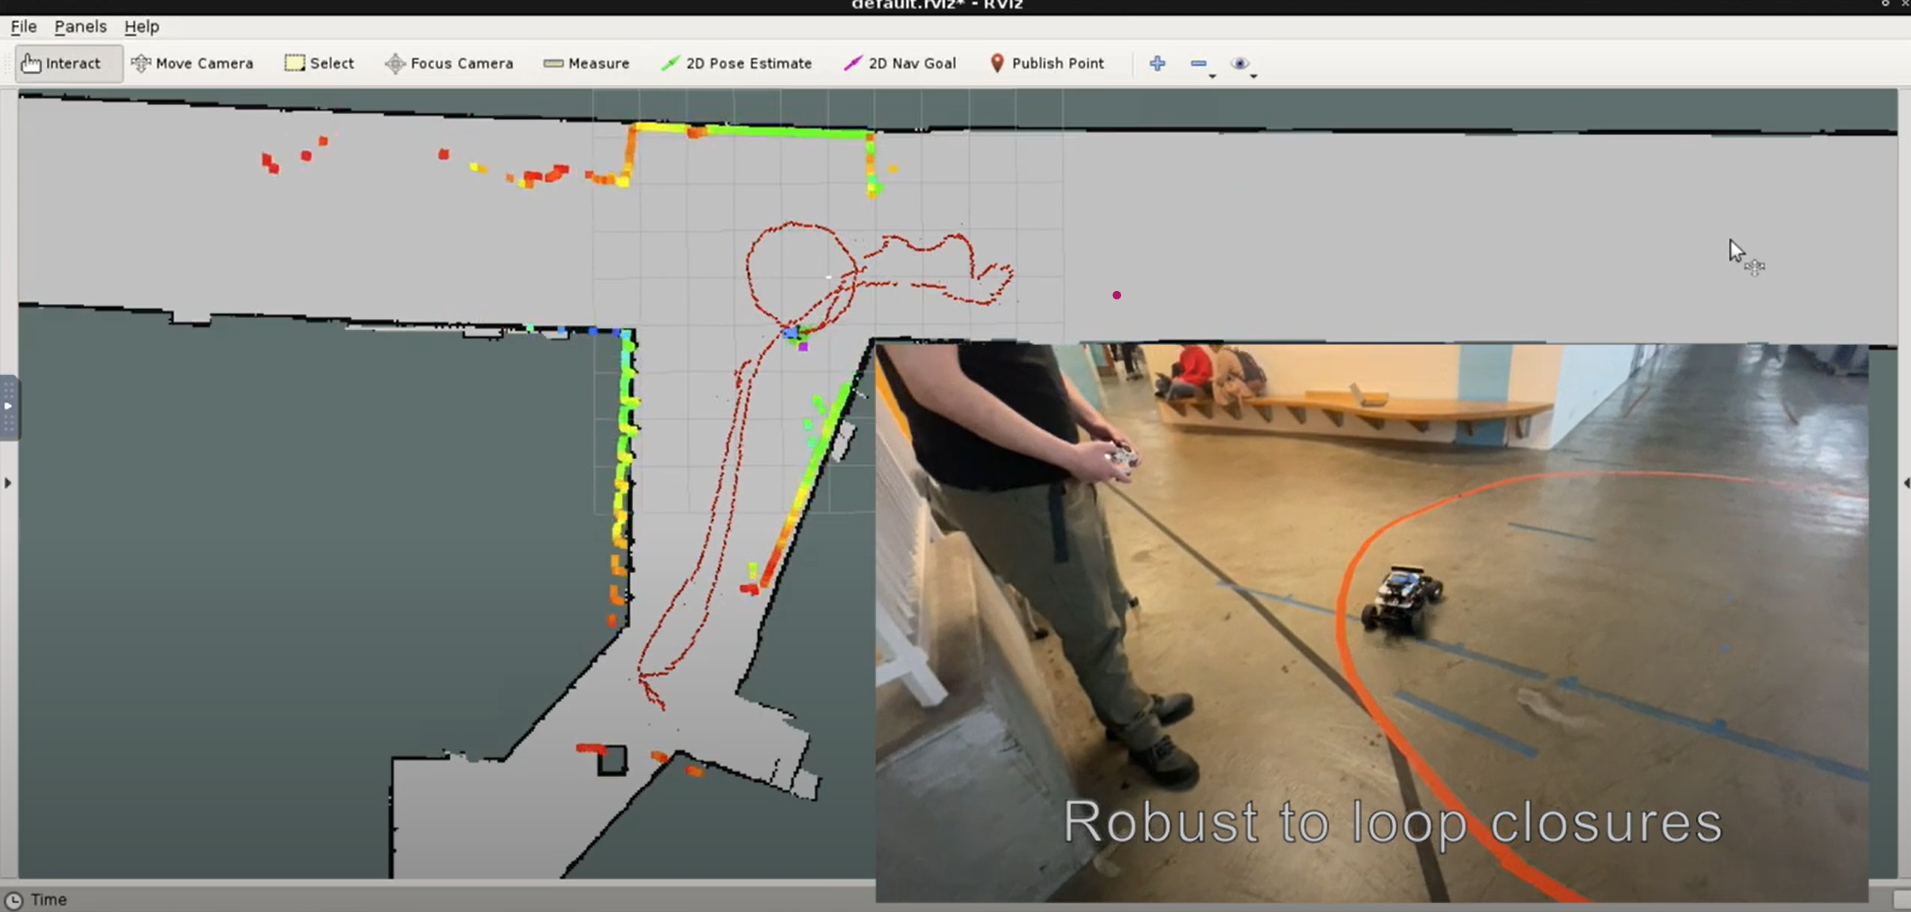
\includegraphics[width=0.8\textwidth]{example_frame.png} % Include the image 
\caption{Example Frame from Demonstration Video. The red dotted line behind the car represents the car's previous estimated positions. The video shows the car's true position. }
\end{center}
\label{workflow}
\end{figure}}

The video shows us that in general our MCL implmentation performs very well! We were able to drive the car around via only viewing its estimated position. In general; the car's slime-trail shows that the car tracks well with respect to it's true position. It is worth noting that the laser scans have a harder time matching to a pose when the robot car is in the uppermost hallway. This is to be expected, as the map given for the Stata basement was created before a series of large crates were placed in the uppermost hallway, thus the map no longr reflects accurate real-world conditions in the uppermost hallway. 


\subsection{Convergence Time}

In order to ensure that our implementation works as expected, we measured the convergence time of our particles (pose estimates). If our implementation were working correctly, we would expect that as we randomly generate poses and resample them, they would converge toward the true position with time. I.e., they would start spread out but converge upon the real location. Thus, we devised a metric to measure the time it takes for particles to converge. \\

\textbf{Definition of Convergence Time}: We sought to evaluate convergence time both on the physical car and in simulation. Recall that a pose $p$ is given by $(x,y,\theta)$. We defined 'unconverged' as when the standard deviation of \textit{one} of $x$, $y$ and $\theta$ is above $x_{up},y_{up},\textrm{ or }\theta_{up}$ respectively. In other words, we consider the particles unconverged when one of $x,y,\theta$ is above a large standard deviation. $x_{up},y_{up},\theta_{up}$ were determined experimentally. We initialized the car in a 'False' location (i.e. we told the car it was in a fake position) and measured the initial standard deviations of the $x,y,\theta$ components of particles across all particles, and defined these as $x_{up},y_{up},\theta$. In practice, the standard deviation is only this high when the car is first initialized in new position or it is fed false data. We defined 'converged' similarly; when \textit{all} of $x,y,\theta$ are below $x_{low},y_{low},\theta_{low}$, where $x_{low},y_{low},\theta_{low}$ were chosen experimentally when the car is confident in its position (i.e. is estimating it's position correctly). Then, convergence time is simply given by the time it takes to go from 'unconverged' to 'converged'. This was measured using $rospy.get\_time()$ in our code. Mathematically, we can write the following expressions to define our measurement metrics: 

\begin{equation}
    \textrm{unconverged}\implies (std(x)>x_{up}) \vee (std(y)>y_{up})\vee (std(\theta)>\theta_{up})
\end{equation}
\begin{equation}
    \textrm{converged}\implies (std(x)<x_{low}) \wedge (std(y)<y_{low})\wedge (std(\theta)<\theta_{low})
\end{equation}
\begin{equation}
    t_{convergence} = t_{converged} - t_{unconverged}
\end{equation}

In simulation, we can get an unconverged state by initializing a new location. In the real world, we could get an unconverged state by feeding the car 'fake' LIDAR scans (i.e. obstructing it's view) and confusing it of it's position. Then we allow the particles to return to a converged state. The results are summarized below in Table 2. 

\begin{center}
    \begin{tabular}{|l|c|c|}
\hline
\textbf{Location}                                           & Real-World (N=6) & Simulation (N=20) \\ \hline
\multicolumn{1}{|c|}{\textbf{Average Convergence Time (s)}} & 0.09             & 0.07              \\ \hline
\end{tabular}
\end{center}
These results tell us that on average, our particles converge in under a 10th of a second both on the real car and in simulation, which is a decently fast rate. However, it is worth noting that the standard deviation of convergence time can be large, as the convergence time depends on a number of random factors including how the particles are initialized, how close he robot's estimated position is to its true position, etc. For example, both on he physical car and in simulation, we saw occasional convergence times on the order of $0.2$ or $0.3$ seconds. So even though the average convergence time is low, in some cases it could be considerably higher.  

\subsection{Cross-Track Error}

Finally, we measured cross-tracking errors in simulation. We listened to the transformation published between $map$ and $base_link$ and compared the translational components to our estimated position in simulation. An example plot of cross track errors obtained by listening to the aforementioned transformation, and publishing the difference with respect to our pose, is show in Figure 6.   

\textbf{\begin{figure}[H]
\begin{center}
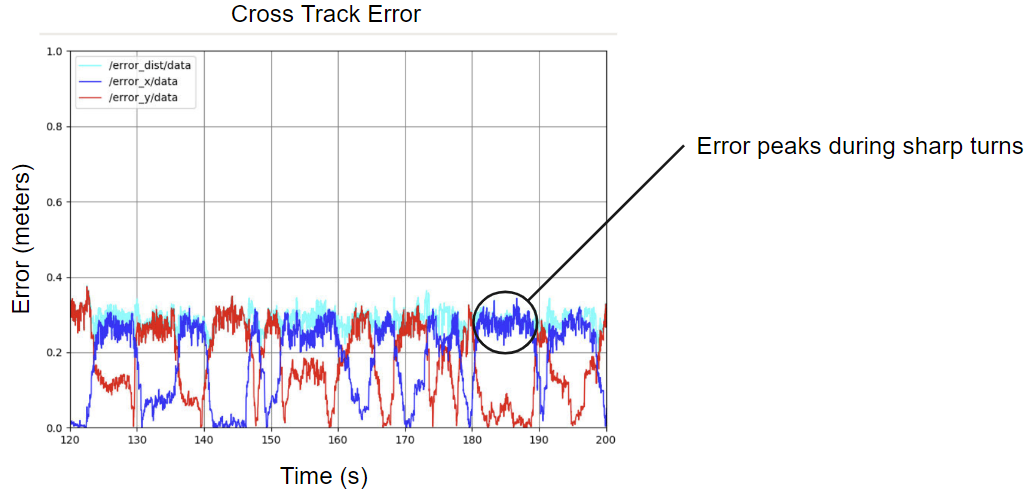
\includegraphics[width=0.8\textwidth]{Cross_Track_Error Simulation.png} % Include the image 
\caption{Cross Track Error Collected over 80 Seconds in Simulation}
\end{center}
\label{workflow}
\end{figure}}
In the above plot, one can view somewhat of a saw-tooth pattern in error. We believe this is primarily due to sharp turns. We manually controlled the car in simulation while collecting the data used in Figure 6, and cross-tracking error would increase for one direction and sometimes decrease for another when the car was rapidly turned. However, we see that the error remains at or below $\approx0.3$ meters for the entirety of the test. This is consistent with our gradescope score of around $0.2-0.25$ meters avg deviation.  

\subsection{Summary} Overall, our car performs well following a line in simulation, has $<0.1$s average convergence rate, and on average has $0.2-0.25$ deviation from a ground truth position. It performs well when tested in the Stata basement, but is sensitive to sharp turns. 




\section{Potential Improvements (Author: Steven Liu)}

Our localization algorithm performs quite well. However, due to time constraints we were not able to do extensive tuning of the parameters used in the motion model and sensor model. As such, it is likely that we could improve performance by a good amount without changing our overall approach.

Speed improvements could also almost certainly be made. The car did not move extremely fast during testing, but as speeds get higher cadences will have to get faster to keep up. There remain some places in our code where we believe we can optimize, in particular by using numpy more extensively.

One notable consistent flaw in our performance is that the estimated pose has a tendency to "understeer" by a small amount; that is, the car thinks it is turning slightly less than it actually is. We were not able to diagnose the underlying cause of this, so it is difficult to speculate what a plausible fix would be.

\section{Conclusion (Author: Jose Soto)}

Overall, our team can confidently say that we developed and implemented Monte Carlo Localization for our vehicle. We were successfully able to implement all three components: the motion model to create odometry estimates, sensor model to explore the probabilities of our particles and the particle filter to refine our odometry estimates using our sensor model. Even after implementing noise, we found our algorithm was able to accurately follow the ground truth solution in simulation. The path to hardware was difficult, requiring several substantial changes, but we were able to reach great localization in our final product. \\

Looking ahead, our team has a few improvements to be made in preparation for our final deliverable at the end of the course which includes: making our localization algorithm more robust to turns, and further improving the latency and refresh rate of the algorithm - especially useful as we plan to traverse the Stata basement at race speeds - which could interfere with the performance of our MCL program. 


\section{Lessons Learned}
%Presents individually authored self-reflections on technical, communication, and collaboration lessons you have learned in the course of this lab.

\subsection{Benjamin Rich}
This lab was probably the most time-consuming one thus far. I learned that it really pays to sit and think and wait until you have a solid grasp of a concept before beginning the code. Rushing to the code prior to truly understand the concept sometimes works in that as you code it you begin to understand it better, but this approach often wastes time. The end result of this lab was really interesting and made the large effort required to get it working totally worth it. 


\subsection{Dinuri Rupasinghe}
I enjoyed this lab because I learned about localization in a more comprehensive, quantitative way. I am glad that I was able to become even more familiar with the general syntax of subscribers and publishers, specifically in our implementation of the particle filter. I am grateful that our team has been proactive in documenting their technical work and will utilize comments and doc strings more often in the future, as I feel that they were extremely helpful for when our team had to work remotely, especially over spring break.

\subsection{Sophia Wang}
This lab was an interesting look into transitioning from software to hardware since threading and seeing how our rates in simulation differed from rates on the robot were both challenging. In terms of debugging, I learned that debugging is most productive in small groups of two to three and also in modules with unit tests. Sometimes, we would gather to debug but found it was hard since only one laptop was connected to the robot at a time, and we were all huddled around a single screen. Overall, I enjoyed this lab and found it very exciting to visualize its results as the racecar traced its own location across the Stata basement.

\subsection{Steven Liu}
This lab was, in terms of technical content, definitely the most interesting of the labs so far; working out the kinks of the motion model and particle filter were gratifying, if quite time-consuming. It's also the first lab for which I was building off of other people's code in a significant way, rather than being the one to provide a first draft of a module, since Dinuri and Sophia got started on the particle filter before I took a serious look at it. This has made me reconsider to some extent how I write code in collaborative environments, specifically with leaving more informative comments and documentation.

\subsection{Jose Soto}
In my opinion this was one of the most technically challenging and interesting labs that we've worked on so far. Spring break falling in the middle of the lab could have posed some communication issues for our team, but I think we handled it well and were able to deliver well despite the circumstances of some members be able to work on the lab while others weren't able to. 
\newpage 
\section{Appendix}


\end{document}